\documentclass[aspectratio=169]{beamer}

% 2   : Introduction (Introduce Idris, The Problem)
% 1.5 : Background (Malfunction, works on the defunctionalised IR, but gets speed ups)
% 1.5 : Compilation of functions (compile functions -> functions to make FFI easier)
% 1   : Compilation of constructors (compile nullary constructors -> integers to make FFI easier)
% 1   : Compilation of laziness (compile laziness -> laziness to make FFI easier) [possible due to Stephen]
% 0.5   : Compilation of floats (compile floats at all) [possible due to Stephen]
% 1 : How Idris does FFIs [1] (Define an FFI value, get a special IO monad)
% 2   : How Idris does FFIs [2] (Define OCaml types and mapping to Idris types as an Idris datatype)
% 2.5 : Functions and IO : Idris represents IO a as `unit -> a`: need to wrap and unwrap
% 2.5 : Modules: records
% 4   : "Demo"git 
% 1   : Conclude + Future work

% Problems:
% 0. Optional and labelled arguments don't translate directly
% 1. Idris's erasure leaves dummy arguments -- especially a problem for passing HO functions (in modules)
% 2. Wrapping and unwrapping IO is (potentially) slow
% 3. Objects?

% Future work:
% 0. Generation of wrappers from .mli (use type providers?)
% 1. Writing more wrappers and writing more programs
% 2. Proper benchmarking

\usepackage{mathpartir}
\usepackage{stmaryrd}
\usepackage{attrib}
\usepackage{rotating}
\usepackage{multirow}
\usepackage{colortbl}
\usepackage{mathpartir}
\usepackage{tikz}
\usepackage[all]{xy}
\usepackage{cmll}

\usepackage{libertine}
\usepackage{newtxmath}
\usepackage{zi4}

\usepackage{smartdiagram}
\usesmartdiagramlibrary{additions}

%\usepackage{euler}
% \usepackage[cm-default]{fontspec}
% \usepackage{xunicode}
% \usepackage{xltxtra}

\newcommand{\TyBool}{\mathsf{Bool}}
\newcommand{\TySet}{\mathsf{Set}}
\newcommand{\TyEl}{\mathsf{El}}

\newcommand{\Ty}{\mathrm{Ty}}
\newcommand{\Tm}{\mathrm{Tm}}
\newcommand{\RTm}{\mathrm{RTm}}
\newcommand{\wk}{\mathsf{wk}}
\newcommand{\proj}{\mathsf{p}}
\newcommand{\vartm}{\mathsf{v}}
\newcommand{\sem}[1]{\llbracket #1 \rrbracket}
\newcommand{\cat}[1]{\mathcal{#1}}
\newcommand{\id}{\mathrm{id}}

\newcommand{\op}{\mathsf{op}}
\newcommand{\Set}{\mathrm{Set}}
\newcommand{\skw}[1]{\mathit{#1}}

\usepackage{mathtools}
\DeclarePairedDelimiter{\floor}{\lfloor}{\rfloor}

\newcommand{\abs}[1]{\lvert #1 \rvert}

\newcommand{\GL}[1]{\mathrm{GL}_#1}
\newcommand{\SynGL}[1]{\mathsf{GL}_#1}
\newcommand{\SE}[1]{\mathsf{SE}_#1}
\newcommand{\SynSE}[1]{\mathsf{SE}_#1}
\newcommand{\Orth}[1]{\mathrm{O}_#1}
\newcommand{\SynOrth}[1]{\mathsf{O}_#1}
\newcommand{\Transl}[1]{\mathrm{T}_#1}
\newcommand{\SynTransl}[1]{\mathsf{T}_#1}
\newcommand{\Scal}{\mathrm{Scal}}
\newcommand{\SynScal}{\mathsf{Scal}}

\newcommand{\tyPrim}[2]{\textup{\texttt{#1}}\langle #2 \rangle}

\newcommand{\sechead}[1]{\textcolor{titlered}{\emph{#1}}}

\newcommand{\typeOfCartSp}[1]{\lbag #1 \rbag}


\def\greyuntil<#1>#2{{\temporal<#1>{\color{black!40}}{\color{black}}{\color{black}} #2}}
\def\greyfrom<#1>#2{{\temporal<#1>{\color{black}}{\color{black!40}}{\color{black!40}} #2}}

\newcommand{\superscript}[1]{\ensuremath{^{\textrm{#1}}}}
\newcommand{\highlight}{\textbf}

\newcommand{\atomprop}{\mathrm}
\newcommand{\true}{\mathbf{T}}
\newcommand{\false}{\mathbf{F}}

\newcommand{\append}{\mathop{+\kern-3pt+}}

\definecolor{titlered}{rgb}{0.8,0.0,0.0}

\newcommand{\hlchange}[1]{\setlength{\fboxsep}{1pt}\colorbox{black!20}{$#1$}}
\newcommand{\altdiff}[3]{\alt<-#1>{#2}{\hlchange{#3}}}

%%%%%%%%%%%%%%%%%%%%%%%%%%%%%%%%%%%%%%%%%%%%%%%%%%%%%%%%%%%%%%%%%%%%%%%%%%%%%%%%
% from http://tex.stackexchange.com/questions/118410/highlight-terms-in-equation-mode
\newlength{\overwritelength}
\newlength{\minimumoverwritelength}
\setlength{\minimumoverwritelength}{0.1cm}
\def\overwrite<#1>#2#3{%
  \settowidth{\overwritelength}{$#2$}%
  \ifdim\overwritelength<\minimumoverwritelength%
    \setlength{\overwritelength}{\minimumoverwritelength}\fi%
  \temporal<#1>{#2}%
    {\stackrel%
      {\begin{minipage}{\overwritelength}%
          \color{red}\centering\small #3\\%
          \rule{1pt}{9pt}%
        \end{minipage}}%
      {\colorbox{red!50}{\color{black}$\displaystyle#2$}}}%
    {\stackrel%
      {\begin{minipage}{\overwritelength}%
          \color{red}\centering\small #3\\%
          \rule{1pt}{9pt}%
        \end{minipage}}%
      {\colorbox{red!50}{\color{black}$\displaystyle#2$}}}}
%%%%%%%%%%%%%%%%%%%%%%%%%%%%%%%%%%%%%%%%%%%%%%%%%%%%%%%%%%%%%%%%%%%%%%%%%%%%%


\setbeamertemplate{navigation symbols}{}
\usecolortheme[rgb={0.8,0,0}]{structure}
\usefonttheme{serif}
%\usefonttheme{structurebold}
\setbeamercolor{description item}{fg=black}

\title{An Idris Foreign Function Interface to OCaml}
\author{Robert Atkey \qquad Ioan Luca\\
  \ \\
  University of Strathclyde, Glasgow, UK}
\date{22nd August 2019}

\begin{document}

\frame{\titlepage}

\newcommand{\youtem}{\quad \textcolor{titlered!80}{---} \quad}

\newcommand{\titlecard}[1]{\begin{frame}%
    \begin{center}%
      \Large \textcolor{titlered}{#1}%
    \end{center}%
  \end{frame}}

\begin{frame}[t]
  \frametitle{Overview}
  \begin{columns}[c]
    \column{.04\textwidth}
    \column{.5\textwidth}
    \begin{block}{What is Idris?}
      \begin{itemize}
        \item General purpose, \textbf{pure} functional language
        \item Has \textbf{dependent types} and a \textbf{strict} semantics
        \item Compiles natively through C, but the runtime is slow
        \item Small library ecosystem
      \end{itemize}
    \end{block}
    \column{.1\textwidth}
    \column{.8\textwidth}
    
\includegraphics[width=.5\textwidth]{logo.png}
  \end{columns}
\end{frame}

\begin{frame}[t]
  \frametitle{Idea}
  \begin{columns}[c]
    \column{.04\textwidth}
    \column{.5\textwidth}
    \begin{itemize}
      \item Compile Idris to OCaml
      \item Build an \textbf{FFI} between the two
      \item Enjoy a high-performance runtime
      \item Get access to a rich ecosystem
    \end{itemize}
    \bigskip
    \begin{itemize}
      \item Goal: make it easier to program in Idris
      \item Non-goal: verify OCaml code
    \end{itemize}
    \column{.1\textwidth}
    \column{.8\textwidth}
    
\includegraphics[width=.5\textwidth]{logo.png}\\~\\
    
\includegraphics[width=.5\textwidth]{ocamllogo.png}
  \end{columns}
\end{frame}


\titlecard{A New OCaml backend for Idris}

\begin{frame}[t]
  \frametitle{Background}
  \begin{columns}[c]
    \column{.04\textwidth}
    \column{.5\textwidth}
    \begin{block}{Malfunction}
      \begin{itemize}
        \item Presented by Stephen Dolan at the ML workshop '16
        \item Untyped program representation
        \item Thin wrapper on top of OCaml's Lambda
        \item S-expressions, so easy to generate
        \item Compiled natively by the OCaml compiler
        \item Programs enjoy \textbf{flambda} optimisations
      \end{itemize}
    \end{block}
    \column{.1\textwidth}
    \column{.8\textwidth}
    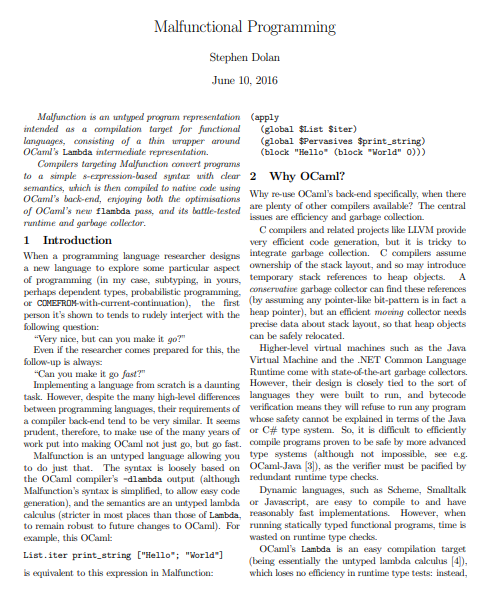
\includegraphics[width=.5\textwidth]{mlfpaper.png}
  \end{columns}
\end{frame}

% \begin{frame}
%   \frametitle{Idris compilation}
%   \begin{center}
%   \smartdiagramset{
%     back arrow disabled=true,
%     additions={
%     additional connections disabled=false,
%     additional item offset=0.85cm,
%     additional item border color=black,
%     additional arrow color=red,
%     additional arrow tip=stealth,
%     additional arrow line width=1pt,
%     additional arrow style=]-latex’,
%     }
%   }
%   \smartdiagramadd[flow diagram:horizontal]{%
%     Idris Source, TT core, Lang, Defunc, Native%
%   }{%
%     above of module1/Low Level, below of module3/High level%
%   }
%   \end{center}
% \end{frame}

\begin{frame}
  \frametitle{Idris compilation via C}
  \centering
  \smartdiagramset{
    back arrow disabled=true,
  }
  \smartdiagram[flow diagram:horizontal]{Idris Source,
    TT core, Lang,  Defunc, Native Code via C}
\end{frame}

\begin{frame}
  \frametitle{Idris compilation via Malfunction after defunctionalisation}
  \centering
  \smartdiagramset{
    back arrow disabled=true,
  }
  \smartdiagram[flow diagram:horizontal]{Idris Source,
    TT core, Lang,  Defunc, Malfunction, Native Code via OCaml}
\end{frame}

\begin{frame}
  \frametitle{Idris compilation via Malfunction before defunctionalisation}
  \centering
  \smartdiagramset{
    back arrow disabled=true,
  }
  \smartdiagram[flow diagram:horizontal]{Idris Source,
    TT core, Lang, Malfunction, Native Code via OCaml}
\end{frame}

\begin{frame}[t]
  \frametitle{Idris-Malfunction}
  \begin{itemize}
    \item Firstly addressed by Stephen
    \item But generates code from a defunctionalised Idris IR
    \item We:
          \begin{itemize}
            \item<2-> Compile Idris functions to OCaml functions
            \item<3-> Compile nullary constructors to integers, instead of
                  boxed integers
                  % \item fixme (what if people ask about the tags limit)
                  % \item implemented a naive lazy evaluation mechanism 
            \item<4-> Implemented some extra primitives
            \item<5-> Compiled Idris laziness to OCaml laziness
            \item<6-> Added support for floats
                  \\ (last 2 possible because of an update to Malfunction)
          \end{itemize}
    \item<7-> Having the same runtime representation for Idris and OCaml
          values, functions and laziness helps with the FFI
    \item<8-> We used a fork of Malfunction that allows access to OCaml
          modules outside the standard library
  \end{itemize}
\end{frame}


% \begin{frame}
%   TODO:
%   \begin{itemize}
%     \item Idris has pluggable backends (C, JavaScript, PHP, ...)
%     \item<2-> Sketch the pipeline (picture?)
%     \item<3-> OCaml is a sensible target
%     \item<4-> Dolan's malfunction backend is quite good
%     \item<5-> But it compiles code after defunctionalisation
%     \item<6-> We:
%           \begin{itemize}
%             \item Use OCaml's closures
%             \item Compile nullary constructors to integers
%           \end{itemize}
%     \item<7-> Challenges
%     \item<8-> Benchmark
%   \end{itemize}
% \end{frame}


\begin{frame}
  \frametitle{Fibonacci --- naive implementation}
  \begin{table}
    \centering
    \begin{tabular}{llll}
           & C      & OCaml  & \\
      real & 5.050s & 3.851s & \\
      user & 5.034s & 3.846s & \\
      sys  & 0.01s  & 0.04s  &
    \end{tabular}
  \end{table}
\end{frame}

\begin{frame}
  \frametitle{Generate the first 500 Pythagorean triplets in a linked list}
  \begin{table}
    \centering
    \begin{tabular}{llll}
           & C      & OCaml  & \\
      real & 3.163s & 0.417s & \\
      user & 3.131s & 0.416s & \\
      sys  & 0.027s & 0.01s  &
    \end{tabular}
  \end{table}
\end{frame}

\begin{frame}
  \frametitle{Balanced binary trees allocation and deallocation}
  \centering
  \begin{tabular}{llll}
         & C       & OCaml   & \\
    real & 58.114s & 18.967s & \\
    user & 44.036s & 18.540s & \\
    sys  & 13.980s & 0.346s  &
  \end{tabular}
\end{frame}

\titlecard{An FFI between Idris and OCaml}

\begin{frame}[t]
  \frametitle{Idris' Foreign Function Interface Interface}

  \begin{displaymath}
    \begin{array}{@{}l}
      \textbf{record}\;\mathrm{FFI}\;\textbf{where} \\
      \quad \textbf{constructor}\;\textsf{MkFFI} \\
      \quad
      \begin{array}{@{}lcl}
        \mathrm{ffi\_types}&:&\textsf{Type} \to \textsf{Type} \\
        \mathrm{ffi\_fn}&:&\textsf{Type} \\
        \mathrm{ffi\_data}&:&\textsf{Type}
      \end{array}
    \end{array}
  \end{displaymath}

  \bigskip
  \pause

  \begin{displaymath}
    \mathrm{foreign} : (f : \mathrm{FFI}) \to \mathrm{ffi\_fn}\,f \to (\mathit{ty} : \textsf{Type}) \to \{\textbf{auto}\;\mathrm{fty} : \mathrm{FTy}\;f\;[]\;\mathit{ty}\} \to \mathit{ty}
  \end{displaymath}

  \bigskip
  \pause

  \begin{displaymath}
    \mathrm{foreign}\;\mathrm{C}\;\textrm{``sin"}\;(\textsf{Float} \to \textsf{IO'}\;\mathrm{C}\;\textsf{Float})
  \end{displaymath}

  \pause

  \begin{displaymath}
    \mathrm{foreign}\;\mathrm{OCaml}\;\textrm{``print\_endline"}\;(\textsf{String} \to \textsf{IO'}\;\mathrm{OCaml}\;())
  \end{displaymath}
\end{frame}

\begin{frame}[t]
  \frametitle{Evidence of Interoperability}

  \begin{displaymath}
    \begin{array}{@{}l}
      \textbf{data}\;\mathrm{FTy} : \mathrm{FFI} \to \mathrm{List}\;\textsf{Type} \to \textsf{Type} \to \textsf{Type}\;\textbf{where} \\
      \quad
      \begin{array}{@{}lcl}
        \textsf{FRet} &:& \textrm{ffi\_types}\;f\; t \to \mathrm{FTy}\;f\;\mathit{xs}\; (\textsf{IO'}\; f\; t) \\
        \textsf{FFun} &:& \textrm{ffi\_types}\; f\; s \to \mathrm{FTy}\; f\; (s :: \mathit{xs})\; t \to \mathrm{FTy}\; f\; \mathrm{xs}\; (s \to t)
      \end{array}
    \end{array}
  \end{displaymath}

  \bigskip

  \begin{displaymath}
    \textsf{FFun}\;\textsf{OCaml\_String}\;(\textsf{FRet}\;\textsf{OCaml\_Unit}) : \mathrm{FTy}\;\mathrm{OCaml}\;[]\;(\textsf{String} \to \textsf{IO'}\;\mathrm{OCaml}\;())
  \end{displaymath}

  \bigskip
  \pause

  \begin{itemize}
  \item Idris generates these witnesses automatically
  \item Every exposed type ends in \textsf{IO'}
  \item Need codes for all OCaml types \ldots
  \end{itemize}
\end{frame}

\begin{frame}[t]
  \frametitle{Representing OCaml types in Idris}

  \begin{displaymath}
    \begin{array}{@{}l}
      \textbf{data}\;\mathrm{OCaml\_Type} : \textsf{Type} \to \textsf{Type}\;\textbf{where} \\
      \quad
      \begin{array}{@{}l@{\quad:\quad}l}
        \textsf{OCaml\_Str}   & \mathrm{OCaml\_Types}\;\mathrm{String} \\
        \textsf{OCaml\_Int}   & \mathrm{OCaml\_Types}\;\mathrm{Int} \\
        \textsf{OCaml\_Float} & \mathrm{OCaml\_Types}\;\mathrm{Double} \\
        \textsf{OCaml\_Bool}  & \mathrm{OCaml\_Types}\;\mathrm{Bool}   \\
        \textsf{OCaml\_Unit}  & \mathrm{OCaml\_Types}\;()              \\
        \textsf{OCaml\_Pair}  & \mathrm{OCaml\_Types}\;a \to \mathrm{OCaml\_Types}\;b \to \mathrm{OCaml\_Types}\;(a,b) \\
        \textsf{OCaml\_List}  & \mathrm{OCaml\_Types}\;a \to \mathrm{OCaml\_Types}\;(\mathrm{List}\;a) \\
        \textsf{OCaml\_Option} & \mathrm{OCaml\_Types}\;a \to \mathrm{OCaml\_Types}\;(\mathrm{Maybe}\;a)\\
        \dots & \dots
      \end{array}
    \end{array}
  \end{displaymath}

\end{frame}

\begin{frame}[t]
  \frametitle{IO Monad vs Pervasive effects}

  In Idris:
  \begin{displaymath}
    \textsf{IO'}\;\mathit{ffi}\;\mathit{ty} \quad \sim \quad \textsf{World} \to \mathit{ty}
  \end{displaymath}
  The \textit{data} associated with the \textsf{World} argument is ``erased''. \\
  But the argument slot still exists...

  \bigskip

  Causes problems when passing functions across the FFI.

  \pause
  \bigskip

  OCaml type:
  \begin{displaymath}
    \mathrm{List.map} : (a \to b) \to a\;\mathrm{list} \to b\;\mathrm{list}
  \end{displaymath}

  Idris type:
  \begin{displaymath}
    (a \to \textsf{IO'}\;\mathrm{OCaml}\;b) \to \mathrm{List}\;a \to \textsf{IO'}\;\mathrm{OCaml}\;(\mathrm{List}\;b)
  \end{displaymath}
  \pause
  Which is effectively:
  \begin{displaymath}
    (a \to \textsf{World} \to b) \to \mathrm{List}\;a \to \textsf{World} \to \mathrm{List}\;b
  \end{displaymath}

\end{frame}

\begin{frame}[t]
  \frametitle{Translating Functions}

  \begin{itemize}
  \item If we stuck to first order, it would be easy \\
    \qquad \textit{(insert an extra ``\textsf{World}'' argument at the end)} \\
    \vspace{1em}
  \item If we knew all the types at compile time, we could statically insert translation code\\
    \qquad \textit{(Idris provides the type information when compiling ``foreign'')} \\
    \vspace{1em}
  \item Want to be able to generate types on the fly when building modules
  \end{itemize}

\end{frame}

\begin{frame}[t]
  \frametitle{Translation}

  Translation functions:
  \begin{displaymath}
    \begin{array}{@{}lcl}
      \textrm{fromOCaml} &:& \textrm{OCaml\_Types}\; a \to a \to a \\
      \textrm{toOCaml} &:& \textrm{OCaml\_Types}\; a \to a \to a
    \end{array}
  \end{displaymath}

  \pause
  \bigskip

  \begin{displaymath}
    \begin{array}{@{}l}
      \mathrm{ocamlCall} : (\mathit{fname} : \mathrm{String}) \to (\mathit{ty} : \textsf{Type}) \to
      \{\textbf{auto}\;\textit{fty} : \textrm{FTy}\;\textrm{OCaml}\; []\; \mathit{ty}\} \to \mathit{ty}\\
      \textrm{ocamlCall}\; \mathit{fname}\; \mathit{ty}\; \{\mathit{fty}\} = \mathrm{fromOCamlFTy}\; \mathit{fty}\; (\mathrm{foreign}\; \mathrm{OCaml}\; \mathit{fname}\; \mathit{ty})
    \end{array}
  \end{displaymath}

  \bigskip
  \pause

  \begin{displaymath}
    \begin{array}{@{}l}
      \textrm{fromOCamlFn}\; (\textsf{OCaml\_FnIO}\; s\; t)\;   f = \\
      \qquad \lambda x \Rightarrow \mathrm{pure}\; (\mathrm{fromOCaml}\; t\; (\mathrm{believe\_me}\; (f\; (\mathrm{toOCaml}\; s\; x)))) \\
      \ \\
      \textrm{toOCamlFn}\; (\textrm{OCaml\_FnIO}\; s\; t)\;   f = \\
      \qquad \lambda x \Rightarrow \textrm{believe\_me}\; (\textrm{toOCaml}\; t\; (\textrm{unsafePerformIO}\; (f\; (\textrm{fromOCaml}\; s\; x))))
    \end{array}
  \end{displaymath}
\end{frame}

\begin{frame}[t]
  \frametitle{Modules}

  {\bf Signatures} 
  \begin{displaymath}
    \textrm{Module}\;[\mathrm{val}\;\textrm{``sleep"}\;(\mathrm{Int64} \to \textsf{IO'}\;\mathrm{OCaml}\;(\mathrm{Lwt}\;()))]
  \end{displaymath}
  \begin{itemize}
  \item A type-level list of string - type pairs
  \end{itemize}

  \bigskip
  \pause

  {\bf Structures}
  \begin{displaymath}
    \textrm{struct}\;[\,\textsf{Let}\,\textrm{``start"} \; \$ \; \lambda () \Rightarrow \mathrm{loop}~4 ]
  \end{displaymath}
  \begin{itemize}
  \item Allocates a block and writes the fields, directed by the type
  \end{itemize}

  \bigskip
  \pause

  {\bf Structure access}
  \begin{displaymath}
    (\textrm{time}\#\textrm{``sleep"})\; (\mathrm{of\_sec}\; 1)
  \end{displaymath}
  \begin{itemize}
  \item Type directed discovery of the index
  \end{itemize}
\end{frame}

\titlecard{Demo}

\begin{frame}[t]
  \frametitle{An Idris / OCaml Foreign Function Interface}

  \begin{itemize}
  \item Improved compilation of Idris via the OCaml backend
  \item An FFI that allows:
    \begin{itemize}
    \item Higher order functions
    \item Simple modules
    \item Some polymorphism
    \end{itemize}
  \end{itemize}

  \bigskip
  \pause

  Limitations / future work:
  \begin{itemize}
  \item Polymorphic signature and structure items
  \item Systematic translation of modules with type members
  \item Better treatment of optional and labelled arguments
  \item Objects?
  \item Generation of wrapper code from \texttt{.mli} files
  \end{itemize}
\end{frame}

\end{document}
